\documentclass[11pt]{beamer}
\newcommand{\R}{\mathbb{R}}
\newcommand{\C}{\mathbb{C}}
\newcommand{\Z}{\mathbb{Z}}
\newcommand{\N}{\mathbb{N}}
\DeclareMathOperator*{\argmin}{arg\,min}
\DeclareMathOperator{\cotan}{cotan}
\DeclareMathOperator{\sinc}{sinc}
\DeclareMathOperator{\Tr}{Tr}
\DeclareMathOperator{\tr}{tr}
\DeclareMathOperator{\Gram}{Gram}
\DeclareMathOperator{\diag}{diag}
\newcommand{\lp}{\left(}
  \newcommand{\rp}{\right)}
\usepackage{blkarray}
\usepackage{multirow}
\usepackage{tikz}
% \usepackage{algorithm2e}
% \usepackage{algorithmic}
\usepackage{float}
\usepackage{framed}
% \usepackage{ulem}
\usetikzlibrary{shapes,arrows}

\newcommand{\lela}{\left \langle}
  \newcommand{\rira}{\right \rangle}
\newcommand{\norm}[1]{\left\lVert#1\right\rVert}
\newcommand{\abs}[1]{\left|#1\right|}

\usepackage{tikz}
\usetikzlibrary{shapes,arrows}
\usepackage[french,english]{babel}
\usepackage[utf8]{inputenc}
\usepackage[T1]{fontenc}
\usepackage{lmodern}
% \usepackage{common}
\usepackage{amsmath,amsfonts,amssymb}
% \usepackage{overpic,boxedminipage}
\usepackage{hyperref}
\usetheme{Warsaw}
\setbeamercolor*{block body alerted}{bg= blue!10}
\setbeamercolor*{block title alerted}{bg= blue!50}
% \usefonttheme{professionalfonts}
\setbeamertemplate{navigation symbols}{}
\setbeamertemplate{headline}{}
\setbeamertemplate{footline}{}
% \setbeamertemplate{blocks}[rounded][shadow=false]
\title[iX_Blue]{SEME 2015: iX-Blue Optimisation de trajectoire pour la navigation Bathymetrique}
\author{Kieran Delamotte, Carlo de Franchis, David Gontier, Antoine Levitt, Fraçois Madiot, Carlo Marcati}
\date{SEME, Vendredi 16 Janvier 2015}
\institute{Sujet proposé par Jérémy Nicola, iXBlue}
% \institute{CEA, DAM, DIF\\Collaboration avec Marc Torrent}
\newcommand{\loja}{\L{}ojasiewicz\xspace}
\begin{document}

\frame{\titlepage}

\frame{\tableofcontents}
\AtBeginSection[]{
  \begin{frame}{Summary}
    \tableofcontents[currentsection, hideothersubsections]
  \end{frame}
}

\section{Présentation du problème}
\subsection{Contexte}
\frame{
  \frametitle{Positionnement}
  \begin{itemize}
  \item Activité principale de iXBlue : conception de système de
    positionnement pour le pétrolier
  \item Interféromètre à base de fibre optique : donne les
    accélérations selon les six degrés de liberté
    \begin{center}
    \resizebox{.3\textwidth}{!}{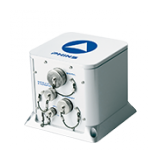
\includegraphics{Images/phins}}
    \resizebox{.5\textwidth}{!}{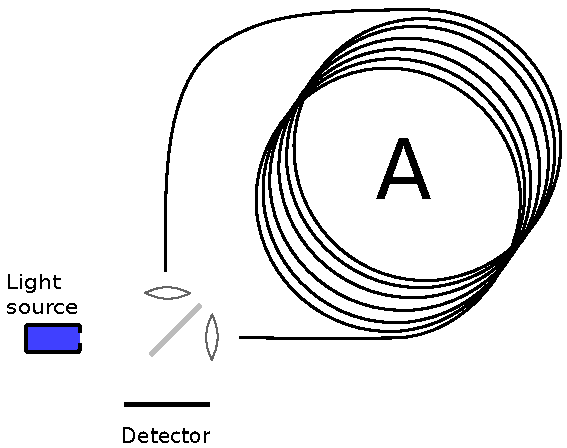
\includegraphics{Images/interferometre}}
  \end{center}
  \end{itemize}

}
\frame{
  \frametitle{Recalage}
  \begin{itemize}
  \item Information locale soumise à dérive. Nécessité d'un recalage
    par des informations globales
  \item Sous-marin : pas possible d'utiliser un GPS
  \item Idée : mesurer le fond marin, et comparer avec des cartes bathymétriques
  \end{itemize}
    \begin{center}
    \resizebox{.6\textwidth}{!}{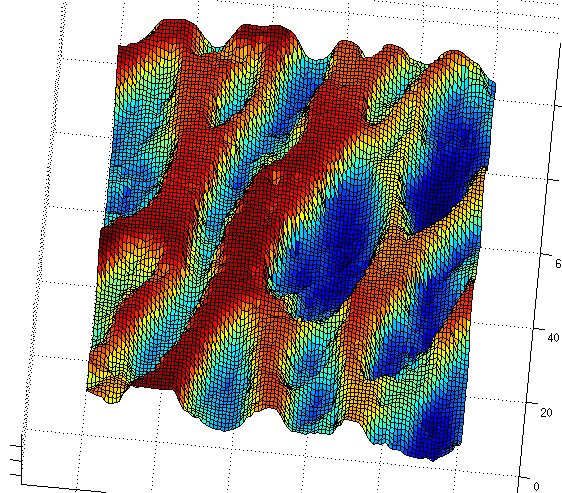
\includegraphics{Images/bathy.png}}
  \end{center}  
}

\frame{
  \frametitle{Choix du chemin}
  \begin{itemize}
  \item Comment aller de $A$ en $B$ de façon précise ?
  \item La ligne droite n'est pas forcément la meilleure
    stratégie. DESSIN ICI
  \end{itemize}
}

\subsection{Notre problème}
\frame{
  \frametitle{Notre problème}
  \begin{center}
    Quel est le chemin de $A$ à $B$ qui minimise l'incertitude en
    $B$ ?
  \end{center}
  \begin{itemize}
  \item Choix du modèle d'incertitudes
  \item Détermination d'une fonction coût
  \item Optimisation de chemin
  \end{itemize}
}

\section{Modélisation et algorithmes de recalage}
\subsection{Modélisation des incertitudes}
\begin{frame}
  \frametitle{Incertitudes}
\begin{itemize}
\item Sources d'incertitude : précision de l'accéléromètre, erreurs
  d'intégration (fréquence finie), erreur numérique (stockage en
  virgule flottante)
\item Dérive de l'estimation de position
\item Modélisation délicate
\item Si on fait une erreur initiale sur l'accélération, dérive en
  $t^{2}$
\item Si on fait une erreur initiale sur la vitesse, dérive en
  $t^{2}$
\item Compensation des erreurs ? Marche aléatoire, dérive en $\sqrt t$
  ? $t^{3/2}$ ? $t^{5/2}$ ?
\item Hors du cadre de l'étude
\item Modèles ad hoc
\end{itemize}
\end{frame}
\subsection{Approche par intervalles}
\begin{frame}

\frametitle{Présentation du problème}


\textcolor{red}{Robot parfait} :
\begin{itemize}
    \item connait parfaitement la trajectoire de $A$ à $B$.
    \item calcule parfaitement $(v_x(t), v_y(t), h(t))$.
\end{itemize}


\begin{figure}[!h]
\begin{center}
    \begin{tikzpicture}[scale =1]

    %% Boite trajectoire
    \draw (0,0) rectangle (7, 6);

    % A et B
    \node at (1, 3.8) {$A$};
    \node at (6, 2.8) {$B$};

    % Obstacle
    \foreach \r in {0.1, 0.2, 0.3, 0.5, 0.8}
    {
        \draw (4, 1.5) circle (\r);
    }

    \draw[line width=1.5]  (1, 3.5) -- (4, 1.5) -- (6, 2.5);
    \only<1> \shade[ball color=red] (1,3.5) circle (.15);
    \only<2> \shade[ball color=red] (4,1.5) circle (.15);
    \only<3> \shade[ball color=red] (6,2.5) circle (.15);



    %% Boite vx
    \draw[->] (8, 4) -> (11, 4);     \draw[->] (8, 4) -> (8, 5.8);
    \node at (8.3, 5.5) {$v_x$}; \node at (11.2, 4) {$t$};

    \only<2-> \draw[red, line width=1.2] (8, 5) -- (10, 5);
    \only<3> \draw[red, line width=1.2] (10,5.4) -- (11, 5.4);

    %% Boite vy
    \draw[->] (8, 2) -> (11, 2);     \draw[->] (8, 2) -> (8, 3.8);
    \node at (8.3, 3.5) {$v_y$}; \node at (11.2, 2) {$t$};

    \only<2-> \draw[red, line width=1.2] (8, 2.5) -- (10, 2.5);
    \only<3> \draw[red, line width=1.2] (10,3.4) -- (11, 3.4);

    %% Boite h
    \draw[->] (8, 0) -> (11, 0);     \draw[->] (8, 0) -> (8, 1.8);
    \node at (8.3, 1.5) {$h$}; \node at (11.2, 0) {$t$};

    \only<2-> \draw[red, line width=1.2] (8, 0.2) -- (9.4, 0.2);
    \only<2-> \draw[red, line width=1.2]  (9.4,0.2) .. controls (9.7,0.2) and (9.8,1.5) .. (10,1.5);
    \only<3> \draw[red, line width=1.2]  (10,1.5) .. controls (10.2,1.5) and (10.3,0.2) .. (10.6,0.2);
    \only<3> \draw[red, line width=1.2] (10.6, 0.2) -- (11, 0.2);


\end{tikzpicture}
\end{center}
\end{figure}


\end{frame}
\subsection{Algorithme de recalage par boites}
Schéma avec trois points

Example avec les trucs blancs
\section{Optimisation de trajectoire}
\subsection{Gloutonne}
\subsection{Dijkstra}
\subsection{Continu}
\section{Future research}
Ellipses ?
\begin{align*}
  \min \sigma_{x}(1) + \sigma_{y}(1)\\
  \sigma_{x}' &= a - b \sigma_{x} (\partial_{x} h)^{2}\\
  \sigma_{x}' &= a - b \sigma_{x} (\partial_{x} h)^{2}
\end{align*}


Modèle isotrope ?

Modèle continu ?
\begin{align*}
  c(\gamma) = \int a |\gamma'^{2}| + \nabla h \cdot \gamma'
\end{align*}


Probas ? Bayésien ?

Feature detection ?
\section{Conclusion}
\end{document}
